\chapter{DFT Calculated Properties}
\label{chapter:dftcalculatedproperties}

\section{QEEOS}

These results were calculated using the QEEOS python program that automatically creates and runs PWscf input files, collects the output files and processes the data.





%%%%%%%%%%%%%%%%%%%%%%%%%%%%%%%%%%%%%%%%%%%%%%%%%%%%%
% Aluminium
%%%%%%%%%%%%%%%%%%%%%%%%%%%%%%%%%%%%%%%%%%%%%%%%%%%%%

\clearpage
\FloatBarrier
\section{FCC Aluminium}

\FloatBarrier
\subsection{DFT Settings for PWscf}

The calculations were performed with the Quantum Espresso PWscf package along with the QEEOS python program.

\begin{table}[h]
\begin{center}
\renewcommand{\arraystretch}{1.2}
\begin{tabular}{c c}
\hline\hline
Setting & Value \\
\hline\hline
ecutwfc (Ry) & 50 \\
ecutrho & 200 \\
smearing (Ry) & 0.04 \\
k-points &  11 11 11 1 1 1  \\
nspin &  0  (Non-magnetic)   \\
pseudopotential &   Al.pbe-nl-kjpaw\_psl.1.0.0.UPF   \\
etot\_conv\_thr & 0.0001 \\
forc\_conv\_thr & 0.001 \\ 
conv\_thr & 1.0D-6 \\ 
diagonalization & david \\ 
mixing\_beta & 0.1 \\ 
mixing\_mode & plain \\ 
\hline\hline
\end{tabular}
\end{center}
\caption{Aluminium DFT settings}
\label{table:alfccdftsettings}
\end{table}



\FloatBarrier
\subsection{Resulting Plots}

\FloatBarrier
\begin{figure}[!htb]
\minipage{0.49\textwidth}
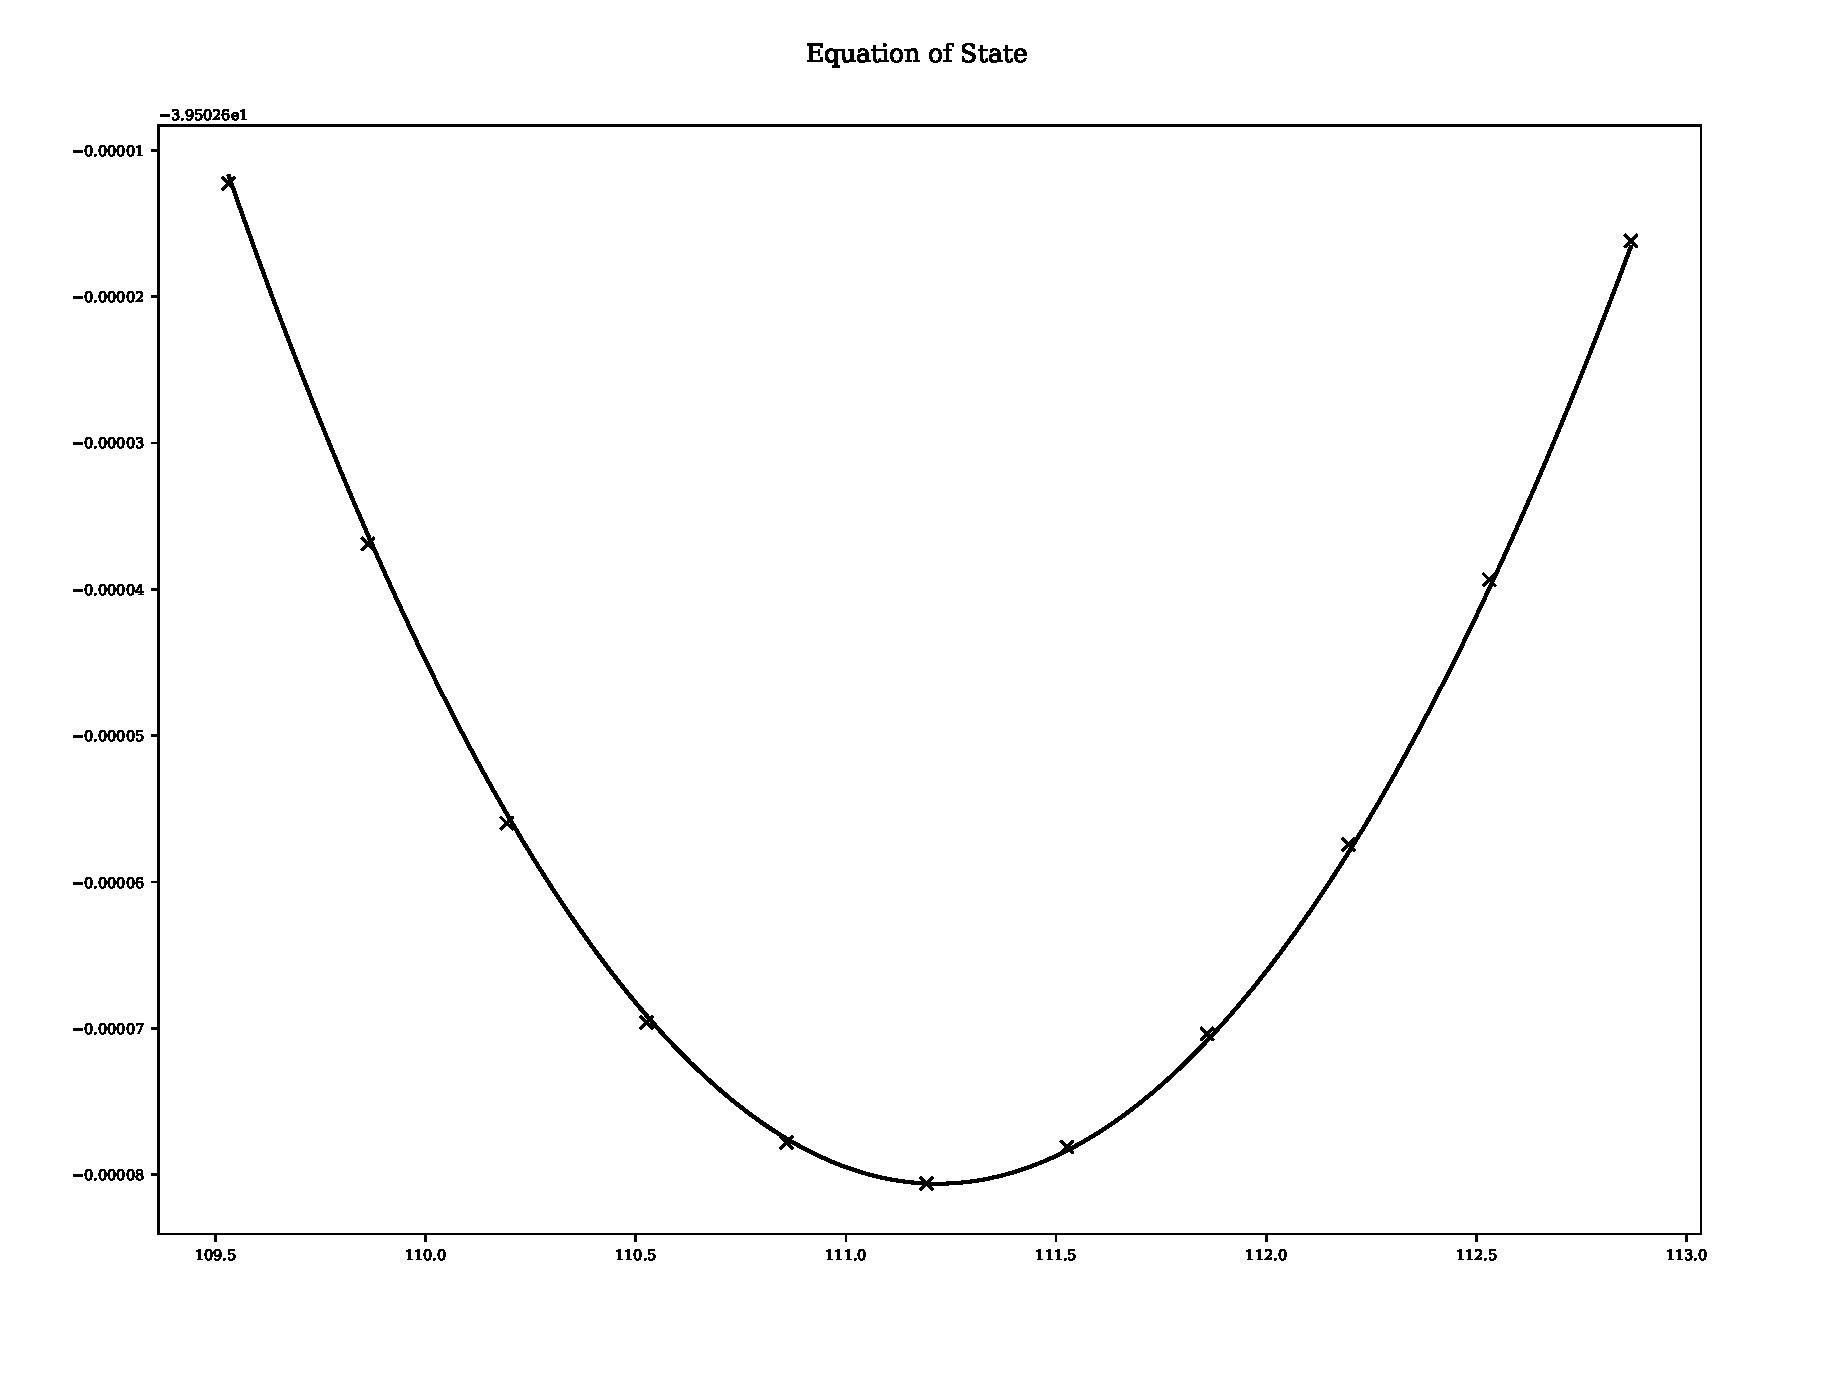
\includegraphics[width=\linewidth]{appendix/dft_property_calculations/fccal/eos.eps}
\caption{Aluminium FCC equation of state plot}
\label{fig:aleosplot}
\endminipage\hfill
\minipage{0.49\textwidth}
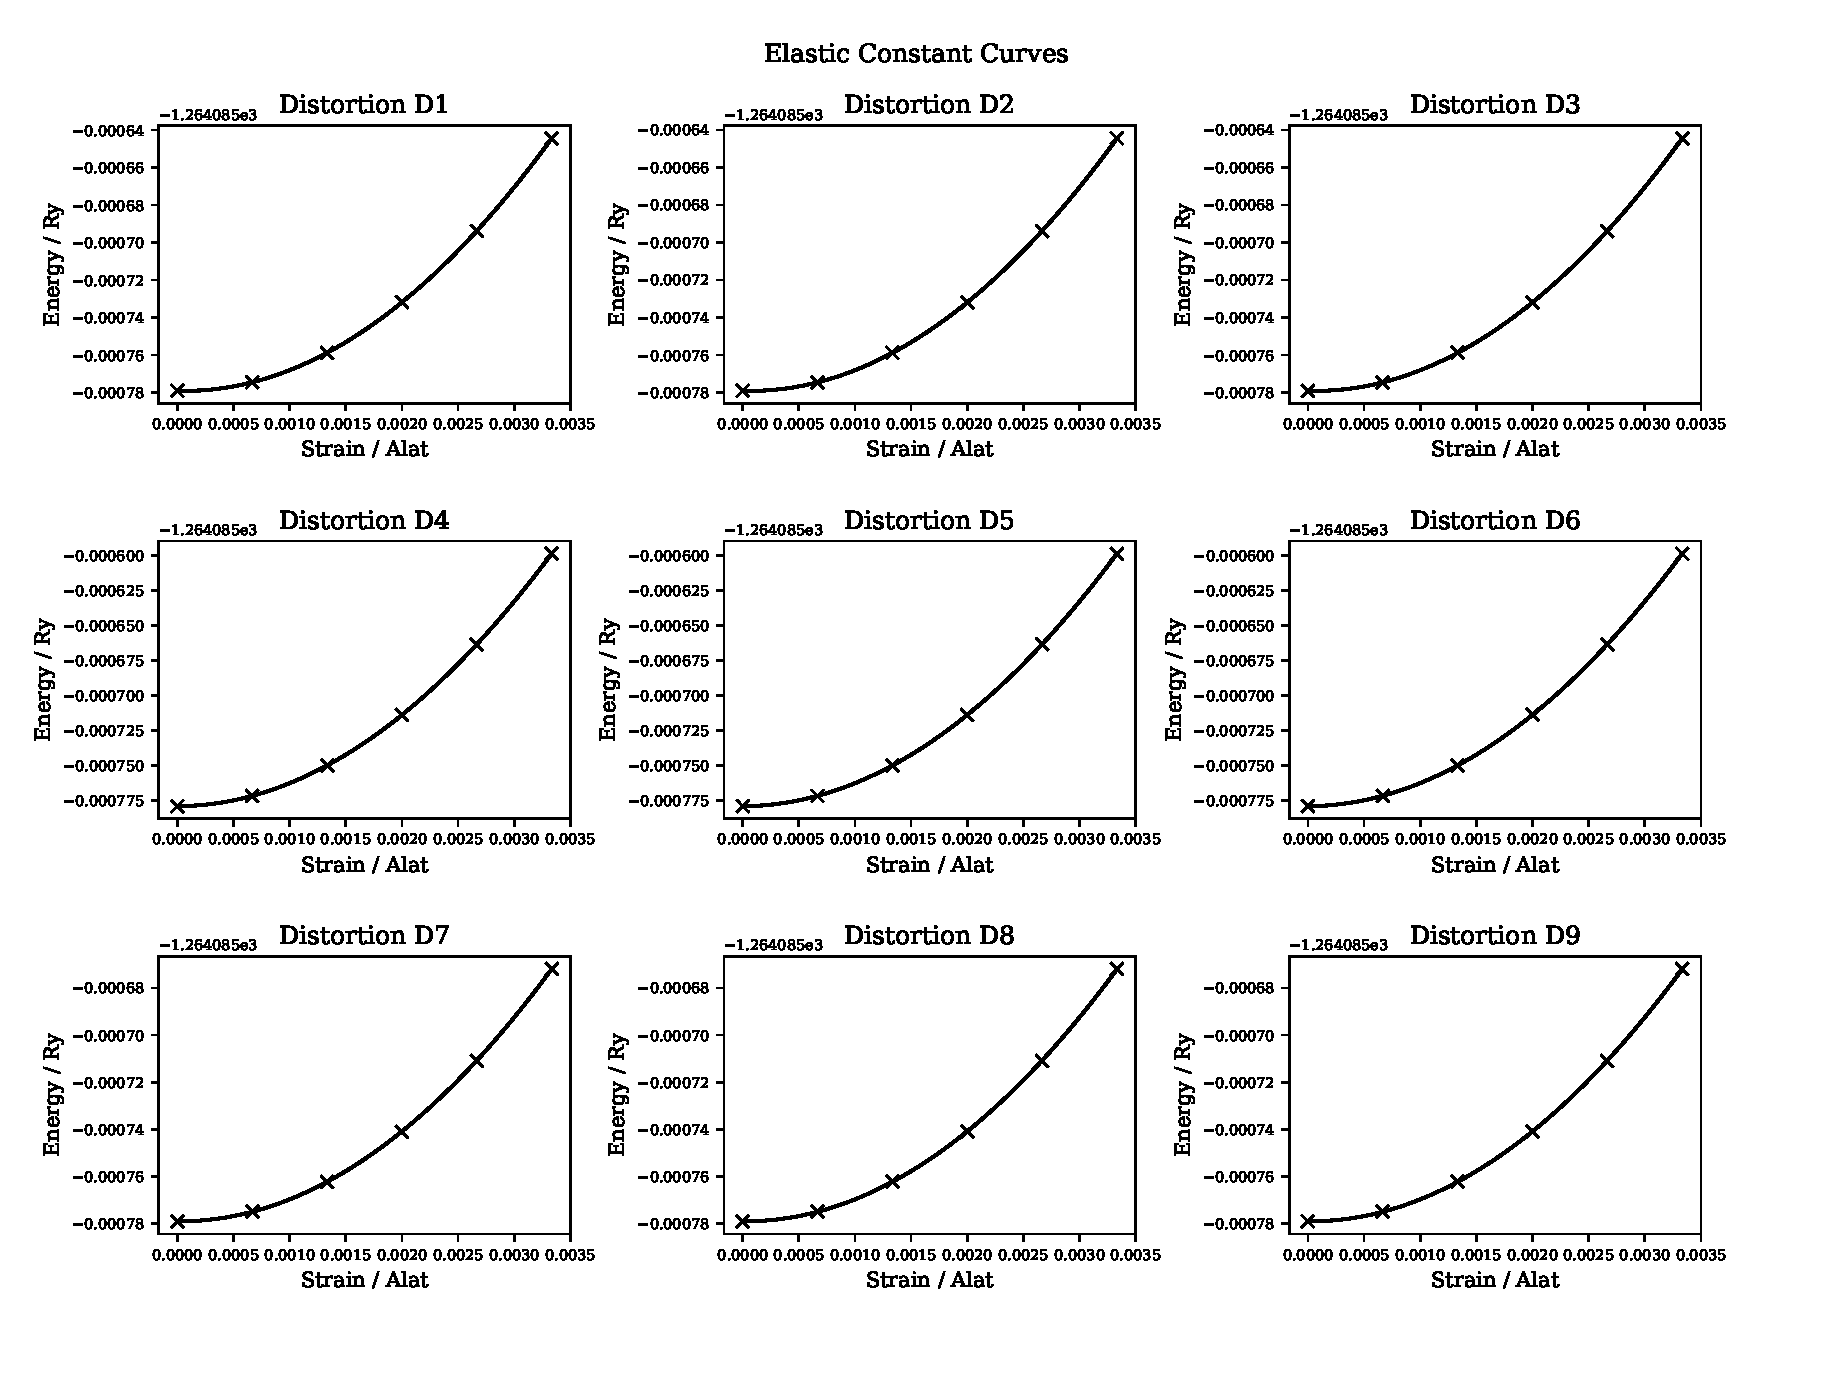
\includegraphics[width=\linewidth]{appendix/dft_property_calculations/fccal/ec.eps}
\caption{Aluminium FCC elastic constants plot}
\label{fig:alecplot}
\endminipage
\end{figure}
\FloatBarrier


\clearpage
\FloatBarrier
\subsection{Aluminium FCC Results File}

\lstinputlisting[style=sOutputFile,caption={Aluminium FCC DFT Calculated Properties}]{appendix/dft_property_calculations/fccal/results.txt}



\FloatBarrier
\subsection{Known and Calculated Values}

\renewcommand{\arraystretch}{1.7}
\begin{table}[ht]
\renewcommand{\arraystretch}{1.2}
\begin{tabular}{lll}
\hline\hline
& Al Experimental & Al DFT (this work)  \\
\hline\hline
Structure                    & Face Centered Cubic & Face Centered Cubic  \\
$a_0$ (Angs)                 & 4.05 Angstrom       & 4.04 Angstrom \\
Nearest Neighbour            & 2.86 Angstrom       & 2.86 Angstrom \\
Basis vectors                & $\begin{bmatrix} 1.0 & 0.0 & 0.0 \\ 0.0 & 1.0 & 0.0 \\ 0.0 & 0.0 & 1.0 \end{bmatrix}$ & $\begin{bmatrix} 1.0 & 0.0 & 0.0 \\ 0.0 & 1.0 & 0.0 \\ 0.0 & 0.0 & 1.0 \end{bmatrix}$ \\
$E_{coh}$ (eV)               & -3.36 eV &  Not Calculated \\
Bulk Modulus $B_0$ (GPA)     & 76  & 77.6 \\
Bulk Modulus $B_{0,r}$ (GPA) & -   & 75.4 \\
Bulk Modulus $B_{0,g}$ (GPA) & -   & 75.4 \\
Young's modulus $E$ (GPA)    & 70  & 81.4 \\
Shear Modulus $G$ (GPA)      & 26  & 30.8 \\
Poisson Ratio $\nu$          & 0.35  & 0.32 \\
Elastic Constants (GPA)      & $\begin{bmatrix} 114 & 62 & 62 & 0 & 0 & 0 \\ 62 & 114 & 62 & 0 & 0 & 0 \\ 62 & 62 & 114 & 0 & 0 & 0 \\ 0 & 0 & 0 & 32 & 0 & 0 \\ 0 & 0 & 0 & 0 & 32 & 0 \\ 0 & 0 & 0 & 0 & 0 & 32 \end{bmatrix}$ & $\begin{bmatrix} 110.9 & 57.7 & 57.7 & 0 & 0 & 0 \\ 57.7 & 110.8 & 57.5 & 0 & 0 & 0 \\ 57.7 & 57.5 & 110.9 & 0 & 0 & 0 \\ 0 & 0 & 0 & 34.0 & 0 & 0 \\ 0 & 0 & 0 & 0 & 34.0 & 0 \\ 0 & 0 & 0 & 0 & 0 & 34.0 \end{bmatrix}$ \\
\hline\hline
\end{tabular}
\caption{FCC Aluminium: Experimental Values vs \acrshort{dft} Calculated Variables}
\label{table:alfccexperimentaldft}
\end{table}



%%%%%%%%%%%%%%%%%%%%%%%%%%%%%%%%%%%%%%%%%%%%%%%%%%%%%
% Iron BCC (no magnetism)
%%%%%%%%%%%%%%%%%%%%%%%%%%%%%%%%%%%%%%%%%%%%%%%%%%%%%

\clearpage
\FloatBarrier
\section{BCC Iron [No Magnetism]}

\FloatBarrier
\subsection{Major DFT Settings}

Ecutwfc: 71 \\
Ecutrho: 430 \\ 
Smearing: 0.04 \\
K-points: 9 9 9 1 1 1 \\
Nspin: 1  (non-polarized calculation) \\
Pseudopotential: Fe.pbe-spn-kjpaw\_psl.1.0.0.UPF \\


\FloatBarrier
\subsection{Equation of State and Elastic Constants}

\FloatBarrier
\begin{figure}[!htb]
\minipage{0.49\textwidth}
\includegraphics[width=\linewidth]{appendix/dft_property_calculations/bccfenomag/eos.eps}
\caption{Iron BCC equation of state plot}
\label{fig:feeosplot1}
\endminipage\hfill
\minipage{0.49\textwidth}
\includegraphics[width=\linewidth]{appendix/dft_property_calculations/bccfenomag/ec.eps}
\caption{Iron BCC elastic constants plot}
\label{fig:feecplot1}
\endminipage
\end{figure}
\FloatBarrier

\clearpage
\FloatBarrier
\subsection{Iron BCC Results File}

\lstinputlisting[style=sOutputFile,caption={Iron BCC DFT Calculated Properties}]{appendix/dft_property_calculations/bccfenomag/results.txt}



%%%%%%%%%%%%%%%%%%%%%%%%%%%%%%%%%%%%%%%%%%%%%%%%%%%%%
% Iron BCC (Ferro)
%%%%%%%%%%%%%%%%%%%%%%%%%%%%%%%%%%%%%%%%%%%%%%%%%%%%%

\clearpage
\FloatBarrier
\section{BCC Iron [Ferromagnetic]}

\FloatBarrier
\subsection{Major DFT Settings}

\begin{table}[h]
\begin{center}
\renewcommand{\arraystretch}{1.2}
\begin{tabular}{c c}
\hline\hline
Setting & Value \\
\hline\hline
ecutwfc (Ry) & 71 \\
ecutrho & 430 \\
smearing (Ry) & 0.04 \\
k-points &  9 9 9 1 1 1   \\
nspin &   0  (Non-magnetic)  and  2 (Collinear Spin)   \\
pseudopotential &   Fe.pbe-spn-kjpaw\_psl.1.0.0.UPF   \\
etot\_conv\_thr & 0.0001 \\
forc\_conv\_thr & 0.001 \\ 
conv\_thr & 1.0D-6 \\ 
diagonalization & david \\ 
mixing\_beta & 0.1 \\ 
mixing\_mode & plain \\ 
\hline\hline
\end{tabular}
\end{center}
\caption{Iron DFT settings}
\label{table:febccdftsettings}
\end{table}


\FloatBarrier
\subsection{Equation of State and Elastic Constants}

\FloatBarrier
\begin{figure}[!htb]
\minipage{0.49\textwidth}
\includegraphics[width=\linewidth]{appendix/dft_property_calculations/bccfe/eos.eps}
\caption{Iron BCC (magnetic) equation of state plot}
\label{fig:feeosplot2}
\endminipage\hfill
\minipage{0.49\textwidth}
\includegraphics[width=\linewidth]{appendix/dft_property_calculations/bccfe/ec.eps}
\caption{Iron BCC (magnetic) elastic constants plot}
\label{fig:feecplot2}
\endminipage
\end{figure}
\FloatBarrier


\clearpage
\FloatBarrier
\subsection{Iron Ferromagnetic BCC Results File}


\lstinputlisting[style=sOutputFile,caption={Iron BCC DFT calculated properties}]{appendix/dft_property_calculations/bccfe/results.txt}



\clearpage
\begin{landscape}
\subsection{Known and Calculated Results}
\renewcommand{\arraystretch}{1.7}
\begin{table}[ht]
\renewcommand{\arraystretch}{1.2}
\begin{tabular}{llll}
\hline\hline
& Fe Experimental & Fe DFT No Magnetism (this work)  & Fe DFT Ferromagnetic (this work) \\
\hline\hline
Structure                    & Body Centered Cubic & Body Centered Cubic  \\
$a_0$ (Angs)                 & 2.86 Angstrom\cite{femendelev} & 2.75 Angstrom & 2.80 Angstrom \\
Nearest Neighbour            & 2.48 Angstrom\cite{femendelev} & 2.38 Angstrom & 2.42 Angstrom \\
Basis vectors                & $\begin{bmatrix} 1.0 & 0.0 & 0.0 \\ 0.0 & 1.0 & 0.0 \\ 0.0 & 0.0 & 1.0 \end{bmatrix}$ & $\begin{bmatrix} 1.0 & 0.0 & 0.0 \\ 0.0 & 1.0 & 0.0 \\ 0.0 & 0.0 & 1.0 \end{bmatrix}$  & $\begin{bmatrix} 1.0 & 0.0 & 0.0 \\ 0.0 & 1.0 & 0.0 \\ 0.0 & 0.0 & 1.0 \end{bmatrix}$\\
$E_{coh}$ (eV)               & -4.32 \cite{femendelev}&  Not Calculated  &  Not Calculated\\
Bulk Modulus $B_0$ (GPA)     & 170  &  287.3    & 239.2 \\
Bulk Modulus $B_{0,r}$ (GPA) & -    &  257.5    & 205.3 \\
Bulk Modulus $B_{0,g}$ (GPA) & -    &  253.7    & 205.3 \\
Young's modulus $E$ (GPA)    & 211  &  -11960.7 & 211.1 \\
Shear Modulus $G$ (GPA)      & 82   &  -643.1   & 79.4 \\
Poisson Ratio $\nu$          & 0.29 &  8.29     & 0.33 \\
Elastic Constants (GPA)      & $\begin{bmatrix} 243 & 145 & 145 & 0 & 0 & 0 \\ 145 & 243 & 145 & 0 & 0 & 0 \\ 145 & 145 & 243 & 0 & 0 & 0 \\ 0 & 0 & 0 & 116 & 0 & 0 \\ 0 & 0 & 0 & 0 & 116 & 0 \\ 0 & 0 & 0 & 0 & 0 & 116 \end{bmatrix}$\cite{femendelev} & $\begin{bmatrix} 63.0 & 329.2 & 315.3 & 0 & 0 & 0 \\ 329.2 & 176.6 & 316.4 & 0 & 0 & 0 \\ 315.3 & 316.5 & 121.7 & 0 & 0 & 0 \\ 0 & 0 & 0 & 176.9 & 0 & 0 \\ 0 & 0 & 0 & 0 & 180.8 & 0 \\ 0 & 0 & 0 & 0 & 0 & 180.0 \end{bmatrix}$ & $\begin{bmatrix} 250.1 & 182.3 & 183.3 & 0 & 0 & 0 \\ 182.3 & 249.1 & 182.9 & 0 & 0 & 0 \\ 183.2 & 182.9 & 251.2 & 0 & 0 & 0 \\ 0 & 0 & 0 & 139.2 & 0 & 0 \\ 0 & 0 & 0 & 0 & 139.7 & 0 \\ 0 & 0 & 0 & 0 & 0 & 139.3 \end{bmatrix}$ \\
\hline\hline
\end{tabular}
\label{tab:feexperimentaldft}
\caption{BCC Iron: Experimental Values vs DFT Calculated Variables}
\label{table:febccexperimentaldft}
\end{table}
\end{landscape}
\clearpage


%%%%%%%%%%%%%%%%%%%%%%%%%%%%%%%%%%%%%%%%%%%%%%%%%%%%%
% Iron FCC (antiferro)
%%%%%%%%%%%%%%%%%%%%%%%%%%%%%%%%%%%%%%%%%%%%%%%%%%%%%

\clearpage
\FloatBarrier
\section{FCC Iron [Antiferromagnetic]}
\label{section:fefccappendix}

\FloatBarrier
\subsection{Major DFT Settings}
\begin{table}[h]
\begin{center}
\renewcommand{\arraystretch}{1.2}
\begin{tabular}{c c}
\hline\hline
Setting & Value \\
\hline\hline
ecutwfc (Ry) & 71 \\
ecutrho & 430 \\
smearing (Ry) & 0.04 \\
k-points &  9 9 9 1 1 1   \\
nspin & 2 (Collinear Spin)   \\
pseudopotential &   Fe.pbe-spn-kjpaw\_psl.1.0.0.UPF   \\
etot\_conv\_thr & 0.0001 \\
forc\_conv\_thr & 0.001 \\ 
conv\_thr & 1.0D-6 \\ 
diagonalization & david \\ 
mixing\_beta & 0.1 \\ 
mixing\_mode & plain \\ 
\hline\hline
\end{tabular}
\end{center}
\caption{Iron DFT settings}
\label{table:fefccdftsettings}
\end{table}



\FloatBarrier
\subsection{Equation of State and Elastic Constants}

\FloatBarrier
\begin{figure}[!htb]
\minipage{0.49\textwidth}
\includegraphics[width=\linewidth]{appendix/dft_property_calculations/fccfe/eos.eps}
\caption{Iron FCC (magnetic) equation of state plot}
\label{fig:feeosplot3}
\endminipage\hfill
\minipage{0.49\textwidth}
\includegraphics[width=\linewidth]{appendix/dft_property_calculations/fccfe/ec.eps}
\caption{Iron FCC (magnetic) elastic constants plot}
\label{fig:feecplot3}
\endminipage
\end{figure}
\FloatBarrier


\clearpage
\FloatBarrier
\subsection{Iron FCC Results File}

\lstinputlisting[style=sOutputFile,caption={Iron FCC DFT Calculated Properties}]{appendix/dft_property_calculations/fccfe/results.txt}



\renewcommand{\arraystretch}{1.7}
\begin{table}[ht]
\renewcommand{\arraystretch}{1.2}
\begin{tabular}{lll}
\hline\hline
& & Iron FCC (this work)  \\
\hline\hline
Structure                    & Face Centered Cubic & Face Centered Cubic  \\
$a_0$ (Angs)                 & - & 3.42 Angstrom \\
Nearest Neighbour            & - & 2.86 Angstrom \\
Basis vectors                & $\begin{bmatrix} 1.0 & 0.0 & 0.0 \\ 0.0 & 1.0 & 0.0 \\ 0.0 & 0.0 & 1.0 \end{bmatrix}$ & $\begin{bmatrix} 1.0 & 0.0 & 0.0 \\ 0.0 & 1.0 & 0.0 \\ 0.0 & 0.0 & 1.0 \end{bmatrix}$ \\
$E_{coh}$ (eV)               & - & -4.26 \\
Bulk Modulus $B_0$ (GPA)     & - & 226.1 \\
Bulk Modulus $B_{0,r}$ (GPA) & -    &  217.3 \\
Bulk Modulus $B_{0,v}$ (GPA) & -    &  226.6 \\
Young's modulus $E$ (GPA)    & - & 356.8 \\
Shear Modulus $G$ (GPA)      & - & 144.8 \\
Poisson Ratio $\nu$          & - & 0.23 \\
Elastic Constants (GPA)      & - & $\begin{bmatrix} 364.6 & 141.6 & 233.8 & 0 & 0 & 0 \\ 141.6 & 298.7 & 130.4 & 0 & 0 & 0 \\ 233.8 & 130.4 & 364.6 & 0 & 0 & 0 \\ 0 & 0 & 0 & 186.3 & 0 & 0 \\ 0 & 0 & 0 & 0 & 266.8 & 0 \\ 0 & 0 & 0 & 0 & 0 & 186.3 \end{bmatrix}$ \\
\hline\hline
\end{tabular}
\caption{Iron FCC: DFT Calculated Properties}
\label{table:fefccexperimentaldft}
\end{table}




%%%%%%%%%%%%%%%%%%%%%%%%%%%%%%%%%%%%%%%%%%%%%%%%%%%%%
% Palladium FCC
%%%%%%%%%%%%%%%%%%%%%%%%%%%%%%%%%%%%%%%%%%%%%%%%%%%%%

\clearpage
\FloatBarrier
\section{FCC Palladium}

\FloatBarrier
\subsection{Major DFT Settings}

\begin{table}[h]
\begin{center}
\renewcommand{\arraystretch}{1.2}
\begin{tabular}{c c}
\hline\hline
Setting & Value \\
\hline\hline
Ecutwfc (Ry) & 71 \\
Ecutrho & 430 \\
Smearing (Ry) & 0.04 \\
K-points &  9 9 9 1 1 1   \\
Nspin &   0  (Non-magnetic)  \\
Pseudopotential &   Pd.pbe-spn-kjpaw\_psl.1.0.0.UPF    \\
etot\_conv\_thr & 0.0001 \\
forc\_conv\_thr & 0.001 \\ 
conv\_thr & 1.0D-6 \\ 
diagonalization & david \\ 
mixing\_beta & 0.1 \\ 
mixing\_mode & plain \\ 
\hline\hline
\end{tabular}
\end{center}
\caption{Palladium DFT settings}
\label{table:pdfccdftsettings}
\end{table}


\FloatBarrier
\subsection{Equation of State and Elastic Constants}

\FloatBarrier
\begin{figure}[!htb]
\minipage{0.49\textwidth}
\includegraphics[width=\linewidth]{appendix/dft_property_calculations/fccpd/eos.eps}
\caption{Palladium FCC equation of state plot}
\label{fig:pdeosplot}
\endminipage\hfill
\minipage{0.49\textwidth}
\includegraphics[width=\linewidth]{appendix/dft_property_calculations/fccpd/ec.eps}
\caption{Palladium FCC elastic constants plot}
\label{fig:pdecplot}
\endminipage
\end{figure}
\FloatBarrier


\clearpage
\FloatBarrier
\subsection{Palladium FCC Results File}

\lstinputlisting[style=sOutputFile,caption={Palladium FCC DFT Calculated Properties}]{appendix/dft_property_calculations/fccpd/results.txt}



\subsection{Known and Calculated Values}


\renewcommand{\arraystretch}{1.7}
\begin{table}[ht]
\renewcommand{\arraystretch}{1.2}
\begin{tabular}{lll}
\hline\hline
& Palladium FCC & Palladium FCC (this work)  \\
\hline\hline
Structure                    & Face Centered Cubic & Face Centered Cubic  \\
$a_0$ (Angs)                 & 3.89  & 3.92  \\
Nearest Neighbour            & 2.75  & 2.77   \\
Basis vectors                & $\begin{bmatrix} 1.0 & 0.0 & 0.0 \\ 0.0 & 1.0 & 0.0 \\ 0.0 & 0.0 & 1.0 \end{bmatrix}$ & $\begin{bmatrix} 1.0 & 0.0 & 0.0 \\ 0.0 & 1.0 & 0.0 \\ 0.0 & 0.0 & 1.0 \end{bmatrix}$ \\
$E_{coh}$ (eV)               & -3.91 &  not calculated \\
Bulk Modulus $B_0$ (GPA)     & 195.5 & 184.4 \\
Bulk Modulus $B_{0,r}$ (GPA) & - & 173.7  \\
Bulk Modulus $B_{0,v}$ (GPA) & - & 173.7  \\
Young's modulus $E$ (GPA)    & 121 & 153.1  \\
Shear Modulus $G$ (GPA)      & 44 & 56.6  \\
Poisson Ratio $\nu$          & 0.39 &  0.35 \\
Elastic Constants (GPA)      & $\begin{bmatrix} 234 & 176.1 & 176.1 & 0 & 0 & 0 \\ 176.1 & 234 & 176.1 & 0 & 0 & 0 \\ 176.1 & 176.1 & 234 & 0 & 0 & 0 \\ 0 & 0 & 0 & 71.2 & 0 & 0 \\ 0 & 0 & 0 & 0 & 71.2 & 0 \\ 0 & 0 & 0 & 0 & 0 & 71.2 \end{bmatrix}$ & $\begin{bmatrix} 218.5 & 151.4 & 151.4 & 0 & 0 & 0 \\ 151.4 & 218.5 & 151.3 & 0 & 0 & 0 \\ 151.4 & 151.3 & 218.5 & 0 & 0 & 0 \\ 0 & 0 & 0 & 80.3 & 0 & 0 \\ 0 & 0 & 0 & 0 & 80.3 & 0 \\ 0 & 0 & 0 & 0 & 0 & 80.3 \end{bmatrix}$ \\
\hline\hline
\end{tabular}
\caption{FCC Palladium: Experimental Values vs DFT Calculated Properties}
\label{table:pdexperimentaldft}
\end{table}



%%%%%%%%%%%%%%%%%%%%%%%%%%%%%%%%%%%%%%%%%%%%%%%%%%%%%
% Palladium FCC
%%%%%%%%%%%%%%%%%%%%%%%%%%%%%%%%%%%%%%%%%%%%%%%%%%%%%

\clearpage
\FloatBarrier
\section{FCC Ruthenium}

\FloatBarrier
\subsection{Major DFT Settings}

Ecutwfc: 71 \\
Ecutrho: 430 \\
Smearing: 0.04 \\
K-points: 9 9 9 1 1 1 \\
Nspin: 1  (non-polarized calculation) \\
Pseudopotential: Ru 101.07 Ru.pbe-spn-kjpaw\_psl.1.0.0.UPF   \\






\FloatBarrier
\subsection{Equation of State and Elastic Constants}

\begin{table}[h]
\begin{center}
\renewcommand{\arraystretch}{1.2}
\begin{tabular}{c c}
\hline\hline
Setting & Value \\
\hline\hline
ecutwfc (Ry) & 71 \\
ecutrho & 430 \\
smearing (Ry) & 0.04 \\
k-points &  9 9 9 1 1 1   \\
nspin & 2 (Collinear Spin)   \\
pseudopotential &   Ru.pbe-spn-kjpaw\_psl.1.0.0.UPF   \\
etot\_conv\_thr & 0.0001 \\
forc\_conv\_thr & 0.001 \\ 
conv\_thr & 1.0D-6 \\ 
diagonalization & david \\ 
mixing\_beta & 0.1 \\ 
mixing\_mode & plain \\ 
\hline\hline
\end{tabular}
\end{center}
\caption{Ruthenium DFT settings}
\label{table:rufccdftsettings}
\end{table}

\clearpage
\FloatBarrier
\subsection{Ruthenium FCC Results File}

\lstinputlisting[style=sOutputFile,caption={Ruthenium FCC DFT Calculated Properties}]{appendix/dft_property_calculations/fccru/results.txt}




\subsection{Calculated Results}

\renewcommand{\arraystretch}{1.7}
\begin{table}[ht]
\renewcommand{\arraystretch}{1.2}
\begin{tabular}{lll}
\hline\hline
& & Ruthenium FCC (this work)  \\
\hline\hline
Structure                    & Face Centered Cubic & Face Centered Cubic  \\
$a_0$ (Angs)                 & - & 3.81 Angstrom \\
Nearest Neighbour            & - & 2.69 Angstrom \\
Basis vectors                & $\begin{bmatrix} 1.0 & 0.0 & 0.0 \\ 0.0 & 1.0 & 0.0 \\ 0.0 & 0.0 & 1.0 \end{bmatrix}$ & $\begin{bmatrix} 1.0 & 0.0 & 0.0 \\ 0.0 & 1.0 & 0.0 \\ 0.0 & 0.0 & 1.0 \end{bmatrix}$ \\
$E_{coh}$ (eV)               & - & -6.62  \\
Bulk Modulus $B_0$ (GPA)     & - & 307.8   \\
Bulk Modulus $B_{0,r}$ (GPA) & - & 303.3 \\
Bulk Modulus $B_{0,v}$ (GPA) & - & 303.3 \\
Young's modulus $E$ (GPA)    & - & 466.9   \\
Shear Modulus $G$ (GPA)      & - & 187.7  \\
Poisson Ratio $\nu$          & - & 0.24   \\
Elastic Constants (GPA)      & - & $\begin{bmatrix} 471.54 & 219.10 & 219.20 & 0 & 0 & 0 \\ 219.10 & 471.55 & 219.20 & 0 & 0 & 0 \\ 219.19 & 219.20 & 471.72 & 0 & 0 & 0 \\ 0 & 0 & 0 & 244.99 & 0 & 0 \\ 0 & 0 & 0 & 0 & 244.97 & 0 \\ 0 & 0 & 0 & 0 & 0 & 244.97 \end{bmatrix}$ \\
\hline\hline
\end{tabular}
\caption{Ruthenium FCC: DFT Calculated Properties}
\label{table:rufccexperimentaldft}
\end{table}






